% Figure 1: MOSAIC pipeline. Build: pdflatex figure1_pipeline.tex  (drawn at \textwidth = 16cm, include at width=\textwidth)
\documentclass[tikz,border=2pt]{standalone}
\usepackage[scaled=0.92]{helvet}
\renewcommand\familydefault{\sfdefault}
\usepackage[T1]{fontenc}
\usetikzlibrary{calc,arrows.meta,decorations.pathreplacing,shapes.geometric}

\definecolor{chartdark}{HTML}{1F4E79}
\definecolor{chartlight}{HTML}{8FA6BC}
\definecolor{chartpale}{HTML}{EEF2F6}
\definecolor{win}{HTML}{D9822B}
\definecolor{winpale}{HTML}{F6DEC4}
\definecolor{ink}{HTML}{2B2B2B}
\definecolor{mute}{HTML}{8A949E}

% schematic per-layer profile (32 bars drawn) (middle layers favoured, as in Fig. heatmap)
\def\profile{0.50,0.40,0.60,0.45,0.50,0.35,0.55,0.40,0.60,0.50,1.20,0.60,0.70,0.80,1.30,1.40,1.20,1.50,1.30,1.40,1.25,0.60,0.50,0.55,0.45,0.60,0.40,0.50,0.45,0.55,0.70,0.80}
\def\refined{0.45,0.40,0.70,0.40,0.45,0.35,0.50,0.40,0.55,0.45,1.35,0.55,0.65,0.95,1.35,1.45,1.10,1.60,1.40,1.45,1.15,0.55,0.45,0.50,0.40,0.55,0.40,0.45,0.40,0.50,0.75,0.85}

\newcommand{\cardw}{3.4}
\newcommand{\cardh}{4.2}
\newcommand{\gap}{0.8}

% \card{index 0-3}{stage label}{title}{description}
\newcommand{\card}[4]{%
  \pgfmathsetmacro{\x}{#1*(\cardw+\gap)}
  \begin{scope}
    \clip[rounded corners=4pt] (\x,0) rectangle ++(\cardw,\cardh);
    \fill[white] (\x,0) rectangle ++(\cardw,\cardh);
    \fill[chartpale] (\x,0) rectangle ++(\cardw,1.25);
    \fill[chartdark] (\x,\cardh-0.62) rectangle ++(\cardw,0.62);
  \end{scope}
  \draw[chartlight, line width=0.6pt, rounded corners=4pt] (\x,0) rectangle ++(\cardw,\cardh);
  \node[anchor=west, text=white, font=\scriptsize] at (\x+0.18,\cardh-0.31) {#2};
  \node[anchor=east, text=white, font=\small\bfseries] at (\x+\cardw-0.18,\cardh-0.31) {#3};
  \node[text width=\cardw cm-0.3cm, align=center, font=\scriptsize, text=ink, inner sep=0pt]
       at (\x+\cardw/2,0.625) {#4};
}

\begin{document}
\hyphenpenalty=10000\exhyphenpenalty=10000
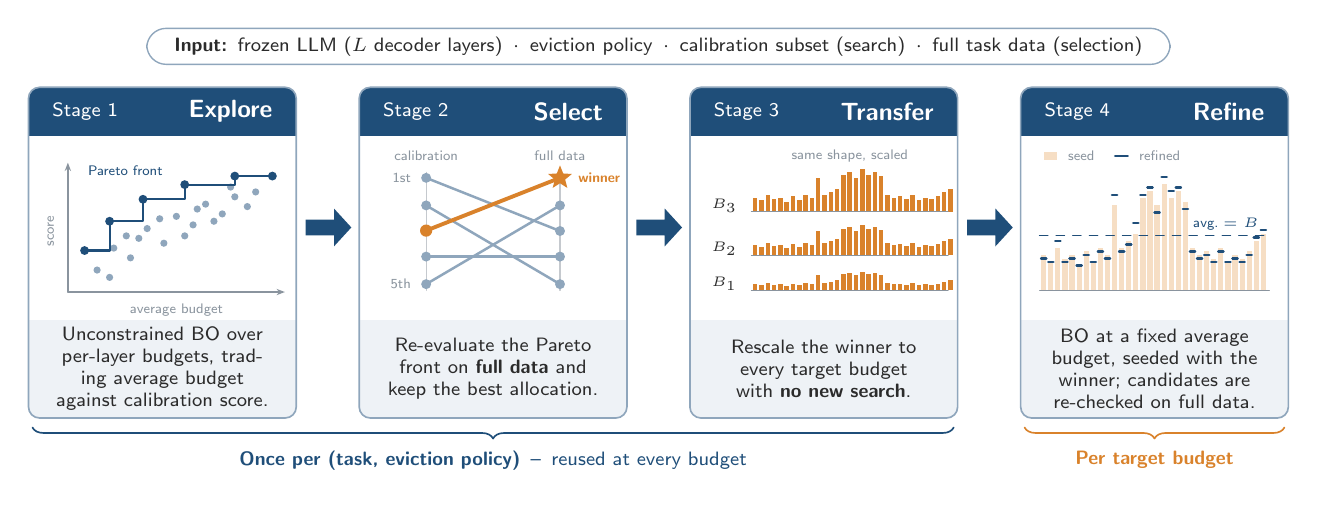
\begin{tikzpicture}[line cap=round, line join=round]

% ---------------- input strip ----------------
\node[draw=chartlight, fill=white, rounded corners=7pt, line width=0.5pt, inner xsep=10pt, inner ysep=3pt,
      font=\scriptsize, text=ink] (in) at (8,4.72)
  {\textbf{Input:}\enspace frozen LLM ($L$ decoder layers)\enspace$\cdot$\enspace eviction policy\enspace$\cdot$\enspace calibration subset (search)\enspace$\cdot$\enspace full task data (selection)};

% ---------------- cards ----------------
\card{0}{Stage 1}{Explore}{Unconstrained BO over per-layer budgets, trading average budget against calibration score.}
\card{1}{Stage 2}{Select}{Re-evaluate the Pareto front on \textbf{full data} and keep the best allocation.}
\card{2}{Stage 3}{Transfer}{Rescale the winner to every target budget with \textbf{no new search}.}
\card{3}{Stage 4}{Refine}{BO at a fixed average budget, seeded with the winner; candidates are re-checked on full data.}

% ---------------- flow arrows between cards ----------------
\foreach \i in {0,1,2}{
  \pgfmathsetmacro{\ax}{\i*(\cardw+\gap)+\cardw+0.12}
  \fill[chartdark] (\ax,2.52) -- ++(0.36,0) -- ++(0,0.14) -- ++(0.22,-0.24) -- ++(-0.22,-0.24) -- ++(0,0.14) -- ++(-0.36,0) -- cycle;
}

% ================= Stage 1 visual: Pareto front =================
\begin{scope}[shift={(0.5,1.6)}, x=2.65cm, y=1.55cm]
  \draw[-{Stealth[length=3pt]}, mute, line width=0.5pt] (0,0) -- (1.04,0);
  \draw[-{Stealth[length=3pt]}, mute, line width=0.5pt] (0,0) -- (0,1.06);
  \node[font=\tiny, text=mute, anchor=north] at (0.52,-0.02) {average budget};
  \node[font=\tiny, text=mute, anchor=south, rotate=90] at (-0.02,0.5) {score};
  \foreach \px/\py in {0.14/0.18,0.22/0.36,0.30/0.28,0.38/0.52,0.46/0.40,0.52/0.62,0.60/0.55,0.66/0.72,0.74/0.64,
                       0.80/0.78,0.86/0.70,0.20/0.12,0.34/0.44,0.56/0.46,0.70/0.58,0.90/0.82,0.44/0.60,0.62/0.68,0.28/0.46,0.78/0.86}
    \fill[chartlight] (\px,\py) circle (1.3pt);
  \draw[chartdark, line width=0.8pt] (0.08,0.34) -- (0.20,0.34) -- (0.20,0.58) -- (0.36,0.58) -- (0.36,0.76) -- (0.56,0.76) -- (0.56,0.88) -- (0.80,0.88) -- (0.80,0.95) -- (0.98,0.95);
  \foreach \px/\py in {0.08/0.34,0.20/0.58,0.36/0.76,0.56/0.88,0.80/0.95,0.98/0.95}
    \fill[chartdark] (\px,\py) circle (1.6pt);
  \node[font=\tiny, text=chartdark, anchor=west] at (0.05,0.99) {Pareto front};
\end{scope}

% ================= Stage 2 visual: ranking slope chart =================
\begin{scope}[shift={(\cardw+\gap,0)}]
  \node[font=\tiny, text=mute] at (0.85,3.33) {calibration};
  \node[font=\tiny, text=mute] at (2.55,3.33) {full data};
  \draw[mute!50, line width=0.4pt] (0.85,1.62) -- (0.85,3.12);
  \draw[mute!50, line width=0.4pt] (2.55,1.62) -- (2.55,3.12);
  % left rank y -> right rank y  (A..E)
  \foreach \l/\r in {3.05/2.375, 2.70/1.70, 2.05/2.05, 1.70/2.70}
    \draw[chartlight, line width=0.9pt] (0.85,\l) -- (2.55,\r);
  \foreach \l/\r in {3.05/2.375, 2.70/1.70, 2.05/2.05, 1.70/2.70}{
    \fill[chartlight] (0.85,\l) circle (1.8pt); \fill[chartlight] (2.55,\r) circle (1.8pt);}
  \draw[win, line width=1.4pt] (0.85,2.38) -- (2.55,3.05);
  \fill[win] (0.85,2.38) circle (2.2pt);
  \node[star, star points=5, star point ratio=2.3, fill=win, inner sep=0pt, minimum size=9pt] at (2.55,3.05) {};
  \node[font=\tiny\bfseries, text=win, anchor=west] at (2.66,3.05) {winner};
  \node[font=\tiny, text=mute, anchor=east] at (0.78,3.05) {1st};
  \node[font=\tiny, text=mute, anchor=east] at (0.78,1.70) {5th};
\end{scope}

% ================= Stage 3 visual: winner rescaled to several budgets =================
\begin{scope}[shift={(2*\cardw+2*\gap,0)}]
  \foreach \lab/\base/\s in {$B_3$/2.62/0.36, $B_2$/2.07/0.25, $B_1$/1.62/0.16}{
    \node[font=\tiny, text=ink, anchor=east] at (0.72,\base+0.08) {\lab};
    \foreach \v [count=\k from 0] in \profile
      \fill[win] (0.80+\k*0.08,\base) rectangle ++(0.058,\v*\s);
    \draw[mute, line width=0.3pt] (0.78,\base) -- (3.28,\base);
  }
  \node[font=\tiny, text=mute] at (2.03,3.33) {same shape, scaled};
\end{scope}

% ================= Stage 4 visual: seed vs refined at fixed average =================
\begin{scope}[shift={(3*\cardw+3*\gap,0)}]
  \foreach \v [count=\k from 0] in \profile
    \fill[winpale] (0.26+\k*0.09,1.62) rectangle ++(0.066,\v*0.9);
  \foreach \v [count=\k from 0] in \refined
    \draw[chartdark, line width=0.9pt] (0.26+\k*0.09,1.62+\v*0.9) -- ++(0.066,0);
  \draw[mute, line width=0.3pt] (0.24,1.62) -- (3.16,1.62);
  \draw[chartdark, dashed, line width=0.5pt] (0.24,1.62+0.775*0.9) -- (3.16,1.62+0.775*0.9);
  \node[font=\tiny, text=chartdark, anchor=south west, inner sep=1pt] at (2.15,1.62+0.775*0.9+0.03) {avg.\ $=B$};
  \fill[winpale] (0.30,3.28) rectangle ++(0.16,0.1); \node[font=\tiny, text=mute, anchor=west] at (0.48,3.33) {seed};
  \draw[chartdark, line width=0.9pt] (1.20,3.33) -- ++(0.16,0); \node[font=\tiny, text=mute, anchor=west] at (1.38,3.33) {refined};
\end{scope}

% ---------------- braces: what is amortized vs per budget ----------------
\draw[decorate, decoration={brace, amplitude=4pt, mirror}, chartdark, line width=0.6pt]
  (0.05,-0.12) -- (3*\cardw+2*\gap-0.05,-0.12)
  node[midway, below=5pt, font=\scriptsize, text=chartdark] {\textbf{Once per (task, eviction policy)} \,--\, reused at every budget};
\draw[decorate, decoration={brace, amplitude=4pt, mirror}, win, line width=0.6pt]
  (3*\cardw+3*\gap+0.05,-0.12) -- (4*\cardw+3*\gap-0.05,-0.12)
  node[midway, below=5pt, font=\scriptsize, text=win] {\textbf{Per target budget}};

\end{tikzpicture}
\end{document}
